\documentclass[letter,11pt]{article}

\usepackage[spanish,es-nodecimaldot]{babel}
\usepackage[utf8]{inputenc}

\usepackage{lmodern}
\usepackage[T1]{fontenc}
\usepackage{textcomp}

\usepackage{framed}
\usepackage[svgnames]{xcolor}
\colorlet{shadecolor}{Gainsboro!50}

\usepackage[shortlabels]{enumitem}
\usepackage{graphicx}
\usepackage{pstricks}
\usepackage{amsmath}

\usepackage{anysize}
\marginsize{3cm}{2cm}{2cm}{3cm}

\usepackage{fancyhdr}
\usepackage{lastpage}
\pagestyle{fancy}
\fancyhf{}
\fancyhead[LE,RO]{Física Básica II}
\fancyfoot[CO,CE]{\thepage\ de \pageref{LastPage}}

\special{papersize=215.9mm,279.4mm}

\usepackage[
    pdfauthor={Carlos Eduardo Caballero Burgoa},%
    pdftitle={Física Básica II},%
    pdfsubject={Tarea 21},%
    colorlinks,%
    citecolor=black,%
    filecolor=black,%
    linkcolor=black,%
    urlcolor=black,
    breaklinks]{hyperref}
\usepackage{breakurl}

\newcommand{\blankpage}{
\newpage
\thispagestyle{empty}
\mbox{}
\newpage
}

\renewcommand{\arraystretch}{1.2}

\begin{document}

\begin{center}
    {\Large \bf{Tarea \#21}}
\end{center}

Demostrar todos los momentos de inercia notables siguientes:

\begin{enumerate}[label=(\alph*)]
\item Barra uniforme, eje en el centro de masa y perpendicular a su longitud.
\begin{equation*}
    I = \frac{1}{12}\, M\, L^2
\end{equation*}
\item Barra uniforme, eje por un extremo y perpendicular a su longitud.
\begin{equation*}
    I = \frac{1}{3}\, M\, L^2
\end{equation*}
\item Disco uniforme, eje en el centro de masa y perpendicular al disco.
\begin{equation*}
    I = \frac{1}{2}\, M\, R^2
\end{equation*}
\item Disco uniforme, eje con el centro de masa y paralelo al disco.
\begin{equation*}
    I = \frac{1}{4}\, M\, R^2
\end{equation*}
\item Aro o anillo uniforme, eje en el centro de masa y perpendicular al aro.
\begin{equation*}
    I = M\, R^2
\end{equation*}
\item Cilindro macizo uniforme, eje de simetría en el centro de masa.
\begin{equation*}
    I = \frac{1}{2}\, M\, R^2
\end{equation*}
\item Esfera maciza uniforme, eje en el centro de masa.
\begin{equation*}
    I = \frac{2}{5}\, M\, R^2
\end{equation*}
\item Cascarón esférico uniforme, eje en el centro de masa.
\begin{equation*}
    I = \frac{2}{3}\, M\, R^2
\end{equation*}
\end{enumerate}

\newpage
\textbf{Solución:} \\

a) Barra uniforme, eje en el centro de masa y perpendicular a su longitud.

\begin{center}
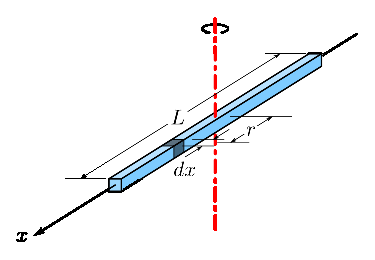
\includegraphics[scale=1.10]{resources/f1.eps}
\end{center}

Dada la ecuación del momento de inercia:

\begin{equation}
    I = \int_{M} r^2\, dm
\label{momentodeinercia1}
\end{equation}

Siendo $r$ equivalente al valor de $|x|$, por tanto:

\begin{equation*}
    r^2 = x^2
\end{equation*}

Asumiendo la distribución homogénea de la masa:

\begin{equation*}
    \lambda = \frac{dm}{dx}
\end{equation*}

Por tanto:

\begin{equation}
    dm = \lambda\, dx
\label{dm1}
\end{equation}

Reemplazando (\ref{dm1}) en (\ref{momentodeinercia1}):

\begin{equation*}
    I = \int_{-L/2}^{L/2} r^2\, \lambda\, dx = \lambda \int_{-L/2}^{L/2} x^2\, dx = \lambda\, \frac{x^3}{3} \Biggr|_{-L/2}^{L/2} = \lambda \left( \frac{(\frac{L}{2})^3}{3} - \frac{(-\frac{L}{2})^3}{3} \right)
\end{equation*}
\begin{equation}
    I = \lambda\, \frac{L^3}{12}
\label{resultado1}
\end{equation}

A partir de la ecuación (\ref{dm1}) sabemos que:

\begin{equation*}
    M = \lambda\, L
\end{equation*}

Despejando $\lambda$ y reemplazando en la ecuación (\ref{resultado1}), obtenemos:

\begin{equation*}
    I = \frac{1}{12} \left( \frac{M}{L} \right) L^3
\end{equation*}

Resultando finalmente:

\begin{equation}
    I = \frac{1}{12}\, M\, L^2
\end{equation}

\newpage
b) Barra uniforme, eje por un extremo y perpendicular a su longitud.

\begin{center}
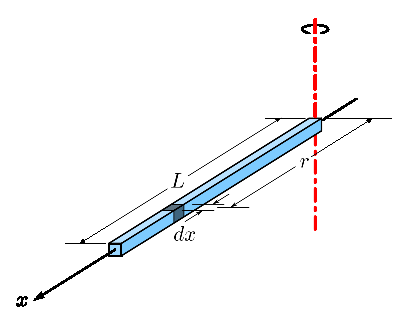
\includegraphics[scale=1.10]{resources/f2.eps}
\end{center}

Dada la ecuación del momento de inercia:

\begin{equation}
    I = \int_{M} r^2\, dm
\label{momentodeinercia2}
\end{equation}

Siendo $r$ equivalente al valor de $|x|$, por tanto:

\begin{equation*}
    r^2 = x^2
\end{equation*}

Asumiendo la distribución homogénea de la masa:

\begin{equation*}
    \lambda = \frac{dm}{dx}
\end{equation*}

Por tanto:

\begin{equation}
    dm = \lambda\, dx
\label{dm2}
\end{equation}

Reemplazando (\ref{dm2}) en (\ref{momentodeinercia2}):

\begin{equation*}
    I = \int_{0}^{L} r^2\, \lambda\, dx = \lambda \int_{0}^{L} x^2\, dx = \lambda\, \frac{x^3}{3} \Biggr|_{0}^{L}
\end{equation*}
\begin{equation}
    I = \lambda\, \frac{L^3}{3}
\label{resultado2}
\end{equation}

A partir de la ecuación (\ref{dm2}) sabemos que:

\begin{equation*}
    M = \lambda\, L
\end{equation*}

Despejando $\lambda$ y reemplazando en la ecuación (\ref{resultado2}), obtenemos:

\begin{equation*}
    I = \frac{1}{3} \left( \frac{M}{L} \right) L^3
\end{equation*}

Resultando finalmente:

\begin{equation}
    I = \frac{1}{3}\, M\, L^2
\end{equation}

\newpage
c) Disco uniforme, eje en el centro de masa y perpendicular al disco.

\begin{center}
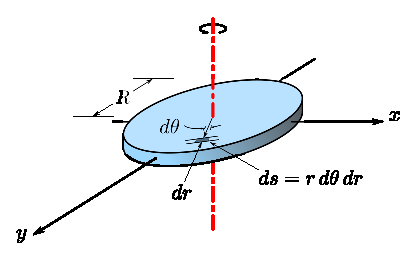
\includegraphics[scale=1.10]{resources/f3.eps}
\end{center}

Dada la ecuación del momento de inercia:

\begin{equation}
    I = \int_{M} r^2\, dm
\label{momentodeinercia3}
\end{equation}

Asumiendo la distribución homogénea de la masa:

\begin{equation*}
    \sigma = \frac{dm}{ds}
\end{equation*}

Usando un diferencial en coordenadas polares obtenemos:

\begin{equation*}
    ds = r\, d\theta\, dr
\end{equation*}

Por tanto:

\begin{equation}
    dm = \sigma\, ds = \sigma\, r\, d\theta\, dr
\label{dm3}
\end{equation}

Reemplazando (\ref{dm3}) en (\ref{momentodeinercia3}):

\begin{equation*}
    I = \int_{S} r^2\, \sigma\, ds = \int_{0}^{R} \int_{0}^{2\pi} r^2\, \sigma\, r\, d\theta\, dr = \sigma \int_{0}^{R} \int_{0}^{2\pi} r^3\, d\theta\, dr = \sigma \int_{0}^{R} ( r^3\, \theta \Biggr|_{0}^{2\pi} )\, dr
\end{equation*}
\begin{equation*}
    I = \sigma \int_{0}^{R} 2\pi\, r^3\, dr = 2\pi\, \sigma \int_{0}^{R} r^3 dr = 2\pi\, \sigma\, \frac{r^4}{4} \Biggr|_{0}^{R} = 2\pi\, \sigma\, \frac{R^4}{4}
\end{equation*}
\begin{equation}
    I = \pi\, \sigma\, \frac{R^4}{2}
\label{resultado3}
\end{equation}

A partir de la ecuación (\ref{dm3}) sabemos que:
\begin{equation*}
    M = \sigma\, S = \sigma\, \pi\, R^2
\end{equation*}

Despejando $\sigma$ y reemplazando en la ecuación (\ref{resultado3}), obtenemos:

\begin{equation*}
    I = \pi\, \left( \frac{M}{\pi\, R^2} \right) \frac{R^4}{2}
\end{equation*}

Resultando finalmente:

\begin{equation}
    I = \frac{1}{2}\, M\, R^2
\end{equation}

\newpage
d) Disco uniforme, eje con el centro de masa y paralelo al disco.

\begin{center}
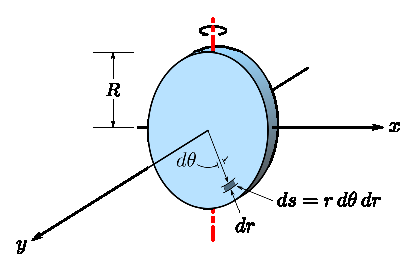
\includegraphics[scale=1.10]{resources/f4.eps}
\end{center}

Dada la ecuación del momento de inercia:

\begin{equation}
    I = \int_{M} r^2\, dm
\label{momentodeinercia4}
\end{equation}

Asumiendo la distribución homogénea de la masa:

\begin{equation*}
    \sigma = \frac{dm}{ds}
\end{equation*}

Usando un diferencial en coordenadas polares obtenemos:

\begin{equation*}
    ds = a\, d\theta\, da
\end{equation*}

Por tanto:

\begin{equation}
    dm = \sigma\, ds = \sigma\, a\, d\theta\, da
\label{dm4}
\end{equation}

Considerando la relación trigonometrica entre las variables $r$ y $a$:

\begin{equation*}
    cos (\theta) = \frac{r}{a}
\end{equation*}

Entonces:

\begin{equation}
    r = a\, cos (\theta)
\label{distancia4}
\end{equation}

Reemplazando (\ref{dm4}) y (\ref{distancia4}) en (\ref{momentodeinercia4}): 

\begin{equation*}
    I = \int_{S} r^2\, \sigma\, ds = \int_{0}^{R} \int_{0}^{2\pi} a^2\, cos^2(\theta)\, \sigma\, a\, d\theta\, da = \sigma \int_{0}^{R} a^3 \int_{0}^{2\pi} cos^2(\theta)\, d\theta\, da
\end{equation*}

Considerando las siguientes propiedades trigonometricas:

\begin{equation*}
    cos^2(x) + sen^2(x) = 1
\end{equation*}
\begin{equation*}
    cos^2(x) - sen^2(x) = cos(2x)
\end{equation*}

Obtenemos:

\begin{equation*}
    2\, cos^2(x) = 1 + cos(2x)
\end{equation*}
\begin{equation}
    cos^2(x) = \frac{1}{2} + \frac{1}{2}\, cos(2x)
\label{trigonometrica4}
\end{equation}

Reemplazando (\ref{trigonometrica4}) en la integral:

\begin{equation*}
    I = \sigma \int_{0}^{R} a^3 \left( \int_{0}^{2\pi} \frac{1}{2} + \frac{1}{2} cos(2\theta) \, d\theta \right) \, da = \sigma \int_{0}^{R} a^3 \left( \frac{1}{2}\, \theta \Biggr|_{0}^{2\pi} + \frac{1}{4} sen(2\theta) \Biggr|_{0}^{2\pi} \right) \, da 
\end{equation*}
\begin{equation*}
    I = \sigma \int_{0}^{R} a^3 \left( \pi + \frac{1}{4} sen(4\pi) - \frac{1}{4} sen(0) \right) \, da = \sigma \int_{0}^{R} a^3 \pi da = \pi\, \sigma \int_{0}^{R} a^3 da = \pi\, \sigma \left( \frac{a^4}{4} \Biggr|_{0}^{R} \right)
\end{equation*}
\begin{equation}
    I = \pi\, \sigma\, \frac{R^4}{4}
\label{resultado4}
\end{equation}

A partir de la ecuación (\ref{dm4}) sabemos que:

\begin{equation*}
    M = \sigma\, S = \sigma\, \pi\, R^2
\end{equation*}

Despejando $\sigma$ y reemplazando en la ecuación (\ref{resultado4}), obtenemos:

\begin{equation*}
    I = \pi\, \left( \frac{M}{\pi\, R^2} \right) \frac{R^4}{4}
\end{equation*}

Resultando finalmente:

\begin{equation}
    I = \frac{1}{4}\, M\, R^2
\end{equation}

\newpage
e) Aro o anillo uniforme, eje en el centro de masa y perpendicular al aro.

\newpage
f) Cilindro macizo uniforme, eje de simetría en el centro de masa.

\newpage
g) Esfera maciza uniforme, eje en el centro de masa.

\newpage
h) Cascarón esférico uniforme, eje en el centro de masa.

\end{document}

